\documentclass[a4paper]{article}

\usepackage[dvipsnames,usenames,svgnames,table]{xcolor}
\usepackage{amsmath}
\usepackage{amssymb}
\usepackage[english]{babel}
\usepackage{caption}
\usepackage{csquotes}
\usepackage{empheq}
\usepackage{enumitem}
\usepackage{float}
\usepackage[bottom]{footmisc}
\usepackage{geometry}
\usepackage{graphicx}
\usepackage{hyperref}
\usepackage{cleveref}
% NOTE: the ordering is important!
\usepackage[toc]{glossaries}
\usepackage[utf8]{inputenc}
\usepackage{multicol}
\usepackage{multirow}
\usepackage{tikz}
\usepackage{titleps}
\usepackage[nottoc,numbib]{tocbibind}
\usepackage{trfsigns}
\usepackage{url}
\usepackage{wrapfig}

% Setup of pagestyle
\newpagestyle{fancypage}{
  \headrule
  \sethead{\MakeUppercase{\thesection\quad \sectiontitle}}{}{\thesubsection\quad \subsectiontitle}
  \setfoot{}{\thepage}{}
}
\settitlemarks{section,subsection,subsubsection}
\pagestyle{fancypage}

% Setup links
\hypersetup{
    linktoc=all,
    citecolor=gray,
    linkcolor=magenta,
    colorlinks=true,
}

\geometry{
 landscape,
 left=15mm,
 right=15mm,
 top=20mm,
 bottom=20mm,
}

\newcommand*\widefbox[1]{\fbox{\hspace{1em}#1\hspace{1em}}}
\newcommand{\circlesign}[1]{
    \mathbin{
        \mathchoice
        {\buildcirclesign{\displaystyle}{#1}}
        {\buildcirclesign{\textstyle}{#1}}
        {\buildcirclesign{\scriptstyle}{#1}}
        {\buildcirclesign{\scriptscriptstyle}{#1}}
    }
}
\newcommand\buildcirclesign[2]{%
    \begin{tikzpicture}[baseline=(X.base), inner sep=0, outer sep=0]
    \node[draw,circle] (X)  {\ensuremath{#1 #2}};
    \end{tikzpicture}%
}
\DeclareMathOperator{\sinc}{sinc}
\DeclareMathOperator{\SNR}{SNR}
\DeclareMathOperator{\Var}{Var}

\graphicspath{ {img/} }

\setlength\columnseprule{0.5pt}
\setlength{\columnsep}{10mm}
\setlength{\parindent}{0mm}
\setlength{\abovecaptionskip}{0pt}
\setlist[1]{itemsep=-0.1em}

\title{\vspace*{\fill}Summary of Cloud Computing at University of Bristol 2018 / 2019\footnote{This is just a simple summary.
I am not responsible for the provided content or anything which belongs to this. If there are any questions please contact me at
bauerflorian13@gmail.com .}}
\author{Florian Bauer\vspace*{\fill}}

\begin{document}
  \begin{titlepage}
    \clearpage
    \maketitle
    \thispagestyle{empty}
  \end{titlepage}

  \begingroup
    \hypersetup{linkcolor=black}
    \clearpage
    \tableofcontents
    \thispagestyle{empty}
  \endgroup
  \pagebreak

  \setcounter{section}{-1}
  \setcounter{page}{1}
  \begin{multicols}{3}

\section*{Lecture 01: Introduction}

\subsection*{Comparison of the internet and electricity network}
\begin{itemize}
    \item starts with everyone has his own (electricity/ computationally power)
    \item connection between every single users grows
    \item ends in an all connected world with only a few big services provided by a small number of providers
    (computationally power goes from the device of the endusers to the cloud, electricity comes from big providers) 
\end{itemize}

\subsection*{Normal Failure}
\begin{itemize}
    \item cloud data centre with $99.999\%$ survival rate
    \item $500 000$ server, probability of $100\%$ of the servers are still running after 3 years is $1\%$.
    \item \textbf{solution}: modular data centres, \textit{servers in container boxes}
\end{itemize}

\subsection*{Essential Characteristics of Cloud Computing}
This definition belongs to NIST's characteristics of Cloud Computing
\begin{itemize}
    \item \textbf{On-demand self service}
    \item \textbf{Broad network access}
    \item \textbf{Ressource pooling}
    \item \textbf{Rapid elasticity}
    \item \textbf{Measured service}
\end{itemize}

\subsection*{A common stratification: *aaS}
\label{subsec:everythingasaservice}
Everything as a Service.
\begin{itemize}
    \item \textbf{SaaS}: \textit{Software as a Service}, for instance: everyone
    \item \textbf{PaaS}: \textit{Platform as a Service}, for instance: \textit{Google App Engine}, \textit{Amazon Appstream}
    \item \textbf{IaaS}: \textit{Infrastructure as a Service}, for instance: \textit{Amazon EC2, S3}, \textit{Google Compute Engine}
\end{itemize}

A small number of companies providing IaaS/PaaS s services. Convergence to an oligopoly of less than five providers seems certain.

\section*{Lecture 02: Coursework}

Just a few informations about the coursework and programming project. May be hopefully not important for the exam...

\section*{L03: Economics of Cloud}

\subsection*{The basic Economics}
\begin{itemize}
    \item \textbf{Cap}ital \textbf{Ex}penditure: \textit{Capex}
    \item \textbf{Op}erating \textbf{Ex}panditure: \textit{Opex}
    \item Capex vs Opex: \textit{Why buy a cow if all you need is the milk?}
\end{itemize}

\subsection*{A typical warehouse scale computer}
\begin{itemize}
    \item \textit{pizzabox} in a \textit{refrigerator} is a server rack
    \item multiple server racks together are a cluster
    \item see \Cref{fig:warehousescalecomputer}
\end{itemize}

\begin{figure}[H]
    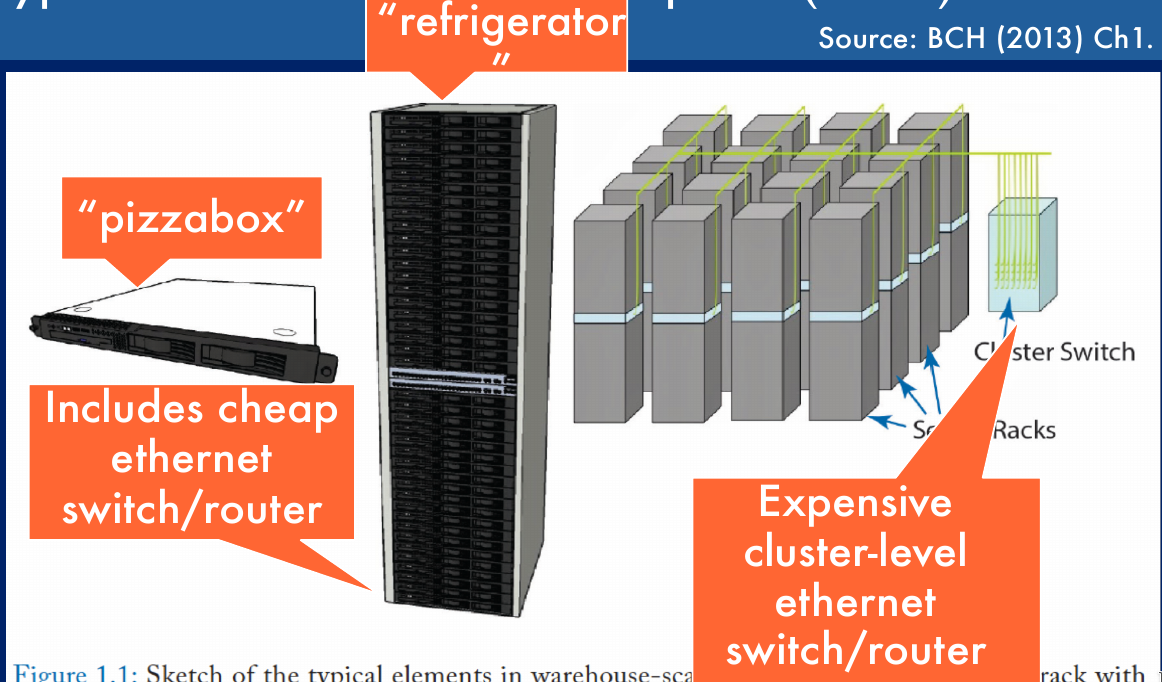
\includegraphics[width=\linewidth]{warehousescalecomputer.png}
    \caption{WSC - Warehouse-scale Computer}
    \label{fig:warehousescalecomputer}
\end{figure}

\subsection*{Energy \& Power Efficiency}
\begin{itemize}
    \item cooling cost are around $42\%$
    \item optimizing the cooling efficiency will lower the overall costs massivley
\end{itemize}

\subsection*{Resume}
\begin{itemize}
    \item there is a lot going on \textit{under the hood of a WSC} (WSC = \textbf{Warehouse-scale Computer})
    \item \textit{prod$>>$dev}: The innovations are made by and in companies not universitys
\end{itemize}

\section*{L05: *aaS}
Definiton see \cref{subsec:everythingasaservice}

\subsection*{Why Xaas or *aaS}
\begin{itemize}
    \item avoiding of \textbf{Undiffertiated Heavy Lifting}
    \item the cloud is an ideal environment providing \textit{scale}, \textit{low cost}, \textit{automation via Infrastructure-as-Code}
\end{itemize}

\begin{figure}[H]
    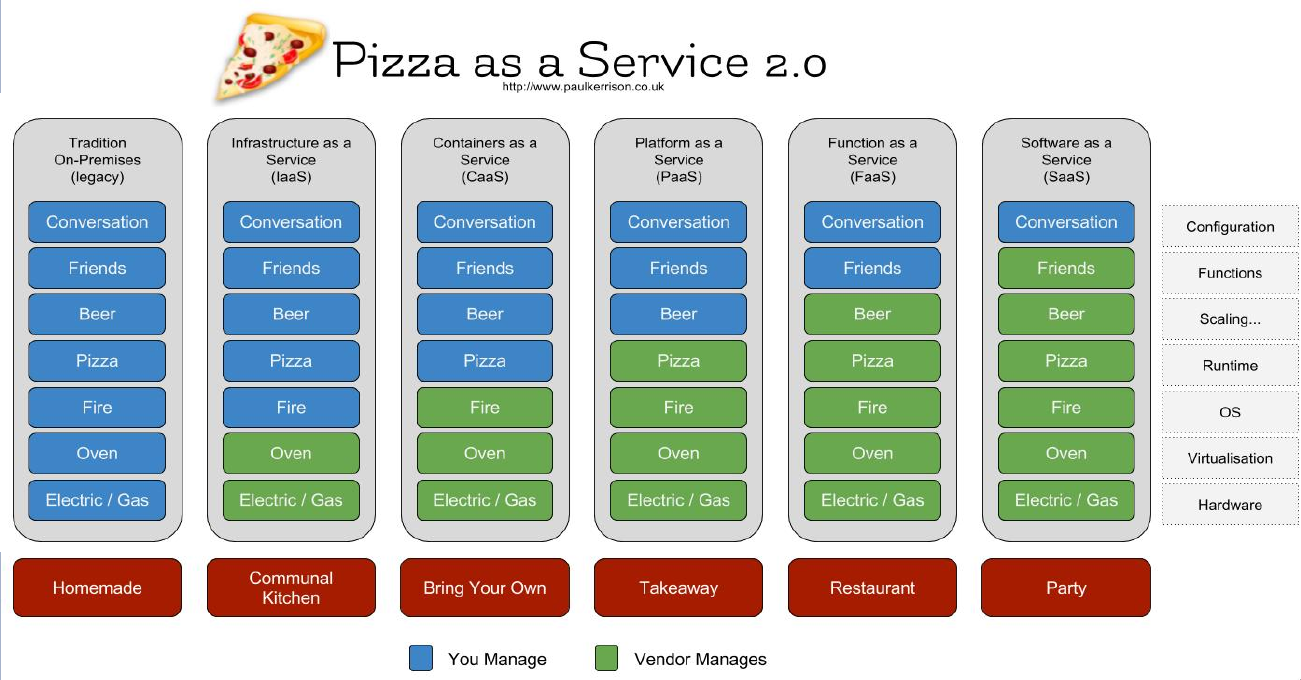
\includegraphics[width=\linewidth]{pizzaserviceexample.png}
    \caption{Pizza as a Service Example for *aaS}
    \label{fig:pizzaservice}
\end{figure}

\subsection*{Structure of AWS Cloud}
\begin{itemize}
    \item \textbf{Availability Zones}: cluster of independent data centres, enables \textbf{fault isolation} and \textbf{high availability}
    \item \textbf{Regions}: entirely independent clouds, consists of a least two \textit{AZ}s, interconnection on global backbone,
    different regions have different costings
\end{itemize}

\subsection*{Which Region should I choose?}
\begin{itemize}
    \item \textbf{Data souvereignty and compilance}: where to store user data?
    \item \textbf{Proximity of users to data}: where are the most of my users? -> lowest latency
    \item \textbf{Services and feature availability}: services and features may vary
    \item \textbf{Cost effectiveness}: each region has different costs (Europe and US are the cheapest)
\end{itemize}

\subsection*{High Availability \& Fault Tolerance}
\textbf{High Availability:}
\begin{itemize}
    \item minimise service downtime by using redundant components
    \item require components in at least two AZs
    \item IaaS may have HA, PaaS usually will have HA
\end{itemize}

\textbf{Fault Tolerance}
\begin{itemize}
    \item ensure no service disruption by using active-active architecture
    \item requires service components in at least three AZs
    \item Iaas is unlikely to offer FT, PaaS some offers FT
\end{itemize}

\subsection*{AWS Storage options}
\begin{itemize}
    \item Elastic Block Storage: SSDs, Magnetic, NAS, Use: OS, Apps
    \item S3: durable object storage, very cheap and big
    \item Instance Storage: on-host storage, very fast, caching
    \item Elastic File Store: shared storage across AZs
\end{itemize}

\subsection*{IaaS vs PaaS}
\begin{itemize}
    \item IaaS mainly used by SysAdmins, PaaS mainly used by Developers
    \item IaaS provides e.g. \textit{VMs},\textit{Storage Services},\textit{Networking}, PaaS provides e.g. hosted databases, \textit{App deployment and managment env.},\textit{test suites}
    \item IaaS lower cloud costs, PaaS lower human costs
\end{itemize}

\section*{L07: Virtualisation, Containers and Container Orchestration}

\subsection*{Virtualisation Basics}
\begin{itemize}
    \item server hardware should be hidden from the user, $\rightarrow$ user sees only guest OS in a VM and not the host OS
    \item Amazon offers different VMs (\textit{AMIs}) with Linux or Windows
    \item VMs are created and run by the \textit{Virtual Machine Monitor (VMM)} aka the \textbf{hypervisor}
    \item VMs can stopped, copied, paused and resumed, which enables \textbf{server consolidation}: compress VMs to freeup servers
\end{itemize}

\subsection*{Types of Virtualisation}
 Have a look at \Cref{fig:vmtypes}

\begin{figure}[H]
    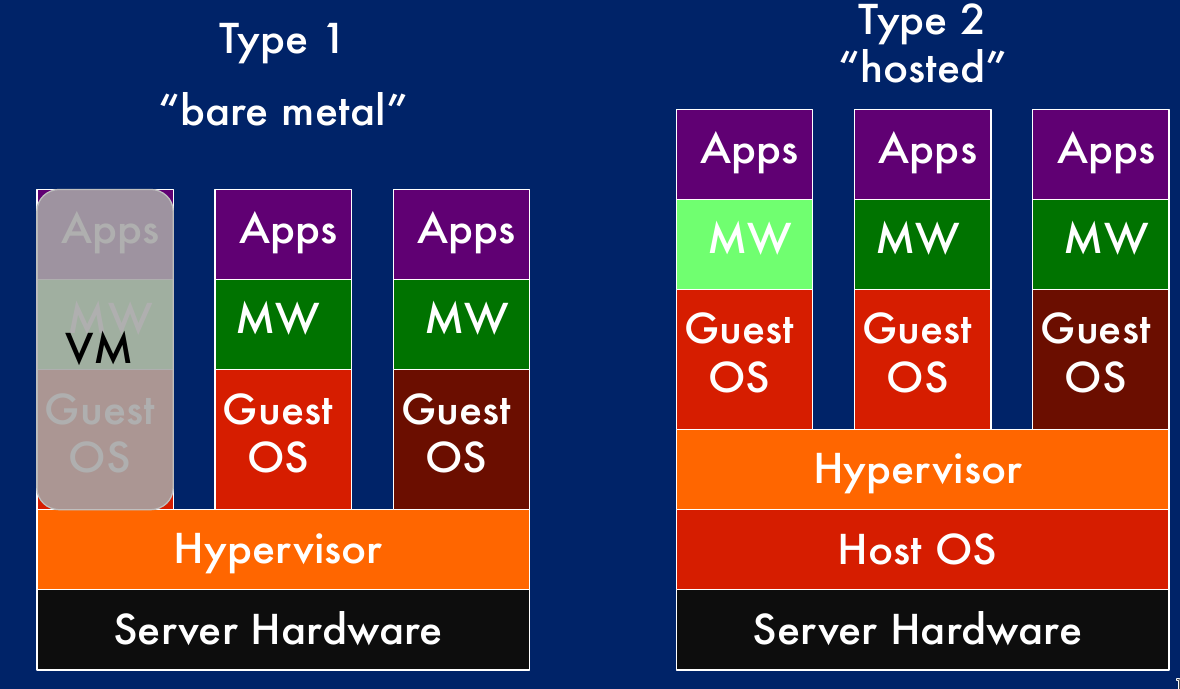
\includegraphics[width=\linewidth]{vmtypes.png}
    \caption{The two different virtualisation types}
    \label{fig:vmtypes}
\end{figure}

\textit{Xen} is an example for Type 1 VMs.

\begin{itemize}
    \item \textbf{Full virtualisation}: complete simulation of underlying guest machine hardware
    \item \textbf{Paravirtualisation}: guest OS can make Syscalls via the hypervisor's API, hypervisor does not simulate hardware
\end{itemize}

\subsection*{Containerisation: Docker}
\begin{itemize}
    \item package and run application in lightweight, isolated environment
    \item Docker runs user processes in a super-isolated execution mode
    \item \textit{operating system level virtualisation} with shared kernel
    \item Advantage: No need to boot a whole VM
    \item Disadvantage: Potentially more insecure than complete virtualisation
\end{itemize}

\textbf{Docker Objects}
\begin{itemize}
    \item \textbf{Images}: read only template with instructions how to create a Docker Container
    \item \textbf{Container}: runnable instance of an  image, but ephemeral $\rightarrow$ all changes not mounted to persistend storage will be lost
\end{itemize}

\begin{figure}[H]
    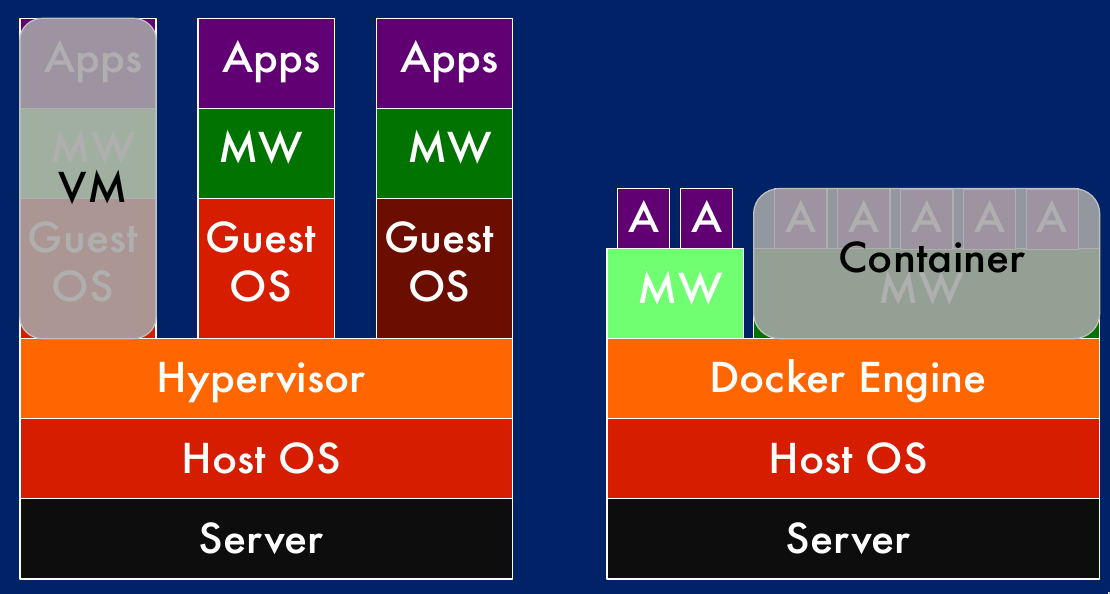
\includegraphics[width=\linewidth]{vmvsdocker.png}
    \caption{VMs vs Docker architecture schema}
    \label{fig:vmvsdocker}
\end{figure}

\subsection*{Container Orchestration: Kubernetes}

\subsubsection*{Motivation}
\begin{itemize}
    \item To run containers at scale needs managment tools
    \item \textbf{(Horizontal) Auto-scaling on demand}
    \item \textbf{Fault Tolerance}
    \item \textbf{Manage Accessibility from the web}
    \item \textbf{update/rollback without downtime}
\end{itemize}

\subsubsection*{Featues of Kubernetes}
\begin{itemize}
    \item \textbf{Automated scaling}
    \item \textbf{Self healing}
    \item \textbf{Horizontal scaling}
    \item \textbf{Service discovery and Load Balancing}
    \item \textbf{Automated Rollbacks/Rollouts}
\end{itemize}

\subsubsection*{Kubernetes Components}
\begin{figure}[H]
    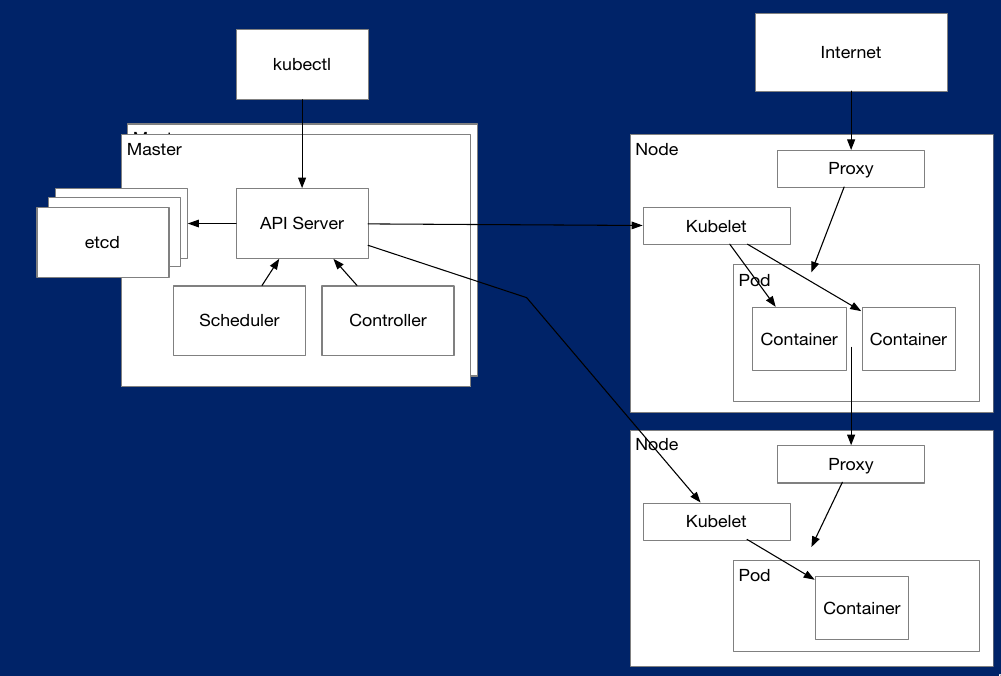
\includegraphics[width=\linewidth]{KubernetesComponents.png}
    \caption{Components of the Kubernetes architecture}
    \label{fig:kubernetescomponents}
\end{figure}

\begin{itemize}
    \item \textbf{Master}: manages the cluster state, subcomponents: \textbf{API Server}, \textbf{Controller}, \textbf{Scheduler}, writes to \textit{etcd} 
    \item \textbf{Nodes}: run work in pods, \textbf{Pods} are the scheduling unit, \textbf{Kubelet} is the agent to communicates with master, \textbf{Kube-proxy} is the network agent
    \item \textbf{Kubeclt}: local cli to controll cluster
    \item \textbf{Etcd}: distributed key-value store
    \item \textbf{Deployments}: \textbf{Replica Sets}, balances the number of running and scheduled pods; deployments provide update to Pods or ReplicaSets
    \item \textbf{Services}: groupings of pods which can be referred by a name, Unique IP and DNS name; Pods in Services are load balanced 
\end{itemize}

\section*{L09: Serverless}

\textbf{Definiton}: \textit{The essence of the serverless trend is the \textbf{absence} of the server concept during software development.}

\subsection*{Abstractions of App Deployment}
\begin{itemize}
    \item \textit{More Abstraction}: more control and trust to given platform
    \item \textit{Less Abstraction}:more undifferentiated heavy lifting
\end{itemize}

\begin{figure}[H]
    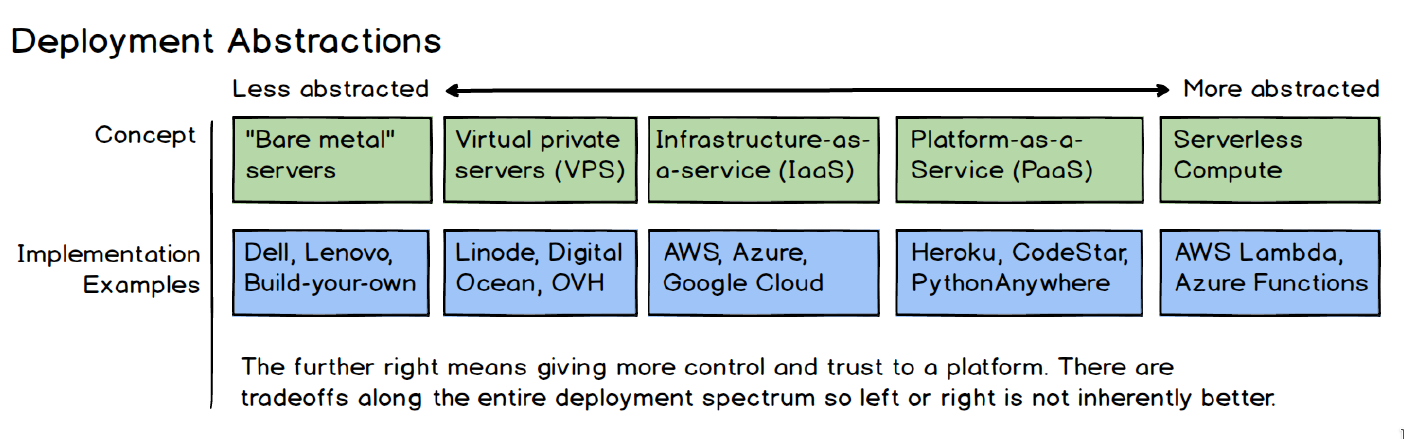
\includegraphics[width=\linewidth]{deploymentabstractions.png}
    \caption{Deployment abstractions: More vs less abstraction}
    \label{fig:deploymentabstractions}
\end{figure}

\subsection*{The four pillars of serverless}
\begin{itemize}
    \item No server managment
    \item Flexible Scaling
    \item High Availability
    \item Never Pay for Idle
\end{itemize}

\subsection*{Serverless FaaS: AWS Lambda}
\begin{itemize}
    \item Triggered by an event
    \item typically invoked in a few ms (warm start)
    \item Cold start issue: code that hasn't been used for a while takes longer to start
\end{itemize}

\begin{figure}[H]
    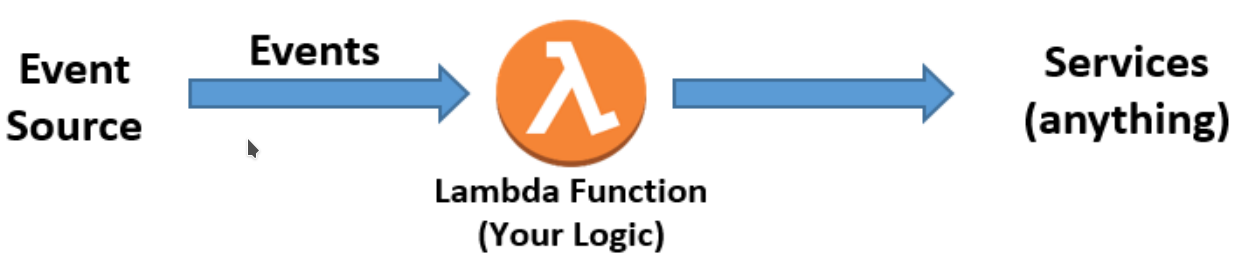
\includegraphics[width=\linewidth]{AWSLambdaTrigger.png}
    \caption{AWS Lambda: Event Triggers}
    \label{fig:awslambda}
\end{figure}

\subsection*{The four stumbling blocks of serverless}
\begin{itemize}
    \item Performance Limitations
    \item Vendor Lock-in
    \item Monitoring and Debugging
    \item Security and Privacy
\end{itemize}

\subsection*{Serverless usecases}
\begin{itemize}
    \item Event-driven data processing (resize uploaded images)
    \item Serverless webapplication (simple 3-tier app)
    \item Mobile  and IoT Apps (Airbnb smart home)
    \item Application Ecosystem (Alexa Skill)
    \item Event Workflow (image recognition and processing)
\end{itemize}

\section*{L11: Scalable Systems}

\subsection*{}
\begin{itemize}
    \item 
\end{itemize}

\section*{L13: MapReduce and GFS/HDFS}

\section*{L14: CAP, Paxos, BGP}

\section*{L15: The Hadoop Ecosystem}

\section*{L16: Spark and In-Memory Methods}

\section*{L17: NoSQL}

\section*{L18: Graph Databases}

\section*{L19: NewSQL $\&$ Event Stream Processing}

\section*{L20: Cloud Security}

\section*{L21: DevOp}

Todo...

\vspace*{\fill}
    \pagebreak
\end{multicols}
\end{document} 
